\section{Empirical Study of Content Between Stack Overflow \& Russian site}

After exploring the users between Stack Overflow and Russian site, this empirical study further analyse the content between two sites from different aspects.

\subsection{Post}
In Q\&A website, users communicate with each other by asking questions and answer questions.
We regards both questions and answers as posts.
In Russian Stack Overflow, there are totally 400,185 posts, and we count how many posts are created by different users.
The results can be seen in Table~\ref{tab:postnumber}.
We can see that more that 6,201 (6.3\%) users who have created more than 10 posts have contributed to 75.9\% content of Russian Stack Overflow.
Due to their importance to the site, we regard these 6,201 users as the core users.

\begin{table}
	\centering
	\caption{Post statics}
	\label{tab:postnumber}
	\begin{tabular}{lrrrr}
		\hline
		\#User Post & \#Post & Post percentage& \#User &User percentage \\
		\hline
		P\_C$>=$2 &372,046&92.9\%&24,908&25.4\%\\
		P\_C$>=$4 &345,543&86.3\%&13,526&13.8\%\\
		P\_C$>=$6 &328,398&82.1\%&9,644&9.8\%\\
		P\_C$>=$8 &314,833&78.7\%&7,537&7.7\%\\
		P\_C$>=$10&303,604&75.9\%&6,201&6.3\%\\
		\hline
	\end{tabular}
\end{table}	

\begin{comment}
Post is the prime part in the content of a Q\&A websites since post is the rising of the question as well as the origin of the answers and comment. It is also a very suitable variable to find the active users and popular topics in the Q\&A website community. Although every user has the right to post a question and add comments, the composition of the knowledge base ought to obey \textcolor{red}{the Pareto Law, which means 20\% of the users make 80\% of the contribution ??where do you find this? any reference or support? in general, literature says power law. how can know 20\% versus 80\%?}.
 
Imagine that a post is a single unit, and millions of posts consist of the knowledge base, and each post includes maybe a lot of answers and comments in the tree structure. 
From Table 1 it is already clear that there are totally 400,185 posts for the Russian Stack Overflow, and using the unique account id to calculate the amount of post for each user on Russian Stack Overflow, the results are presented in Table~\ref{tab:postnumber}. 	



From the table, the static distribution can be easily seen. As mentioned above, with the number of a single user post sum growing, the user proportion decrease. Notice that 6,201 (6.3\%) people from the 98,125 Russian Stack Overflow users who have 10 or more posts contribute 75.9\% of the post amount. These users could be labled as ´ Core User´ in this study representing the ones who have the highest level of contribution. Again, in these 6,201 core users, 1,845 people
are local users while 4,356 people own both main site account and Russian sub-site
account at the same time. In these 4,356 users in the intersection, 1,835 people are
migrants from the Stack Overflow main site. This distribution has been shown in Figure~\ref{fig:reputationTree}.

For the \textcolor{red}{1,676 ??where is this number from? never appear above?} of Core Users who sign up the Stack Overflow account first, which also known as the migrant from the main site, they post 104,448 posts on Russian sub-site that count 26.1\% of the post amount on Russian sub-site. For the \textcolor{red}{2,521 ??where is this number from?} of Core Users who sign up the Russian sub-site account first, which also known as the migrant from the main site, they post 139,275 posts on Russian sub-site that count 34.8\% of the post amount on Russian sub-site. According to the average level, the external users do not dominate the post area. 

\end{comment}

Among these 6201 core users, 4356 of them own both Stack Overflow and Russian Stack Overflow account (seen in Fig~\ref{fig:reputationTree}). 
1835 users registered Stack Overflow first, and created 139,275 posts on Russian Stack Overflow which counts 34.8\% of all posts.
It shows that although many core users may come from Stack Overflow they do not dominate Russian Stack Overflow.
Actually most contributions come from local users in the Russian site.

\begin{figure}
	\centering
	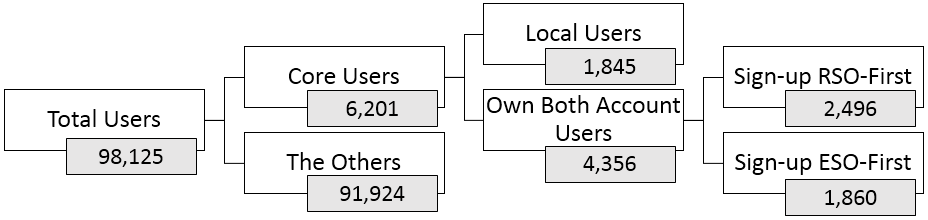
\includegraphics[width = 0.3\textwidth]{figures/usercomponent.png}
	\caption{User components on Russian Stack Overflow \textcolor{red}{CCY:Please draw this figure horizontally to save some space.}}
	\centering
	\label{fig:reputationTree}
\end{figure}

A core user owning both accounts in two sites and registering Stack Overflow first does not necessarily demonstrates that he migrate from Stack Overflow to the Russian one.
To locate users who migrate from Stack Overflow to the Russian one, we define the following formula: 

\textcolor{red}{CCY: This formula seems wrong. It should be that the $\#MainsitePostCountAfterRegistration/TimeLengthAfterRegistration$, so need to re-calculate it.}
\begin{equation}
	f = \frac{\#RussianPostCountAfterRegistration/TimeLengthAfterRegistration}{  \#MainsitePostCountBeforeRegistration /TimeLengthBeforeRegistration}	 
	\label{equ:active}
\end{equation}

The larger value represents the more possibility one user migrate from Stack Overflow to Russian Stack Overflow.
It means that if a core user in Russian Stack Overflow is more likely migrant if he creates fewer posts in Stack Overflow after his registration of the Russian one than that before his registration.

\begin{comment}
Moreover, for the 1,835 of Core Users who sign up the Stack Overflow account first,
according to their frequency of post activity, it can be also concluded that they are still
spending more time and concentrate on the Stack Overflow main site. The formula of
judging a migrant is Formula~\ref{equ:active}. If the f value is greater than 1, the user transferred his or her main active area to the new site.
\end{comment}

	
Assume that a reasonable range for the unchanged active level that is 0.8 to \textcolor{red}{1.2 ??why not 1?} for f, the results in Table~\ref{tab:table3} reveal that more than half of those active users from the main site tend to be more active in a multilingual sub-site. Although they are from another site, they make a lot of contribution and seem to be like using the new sub-site regularly. The conclusion of the research on post aspect is the multilingual community has a group of users as backbone so that the community is not dominated by the users from the Stack Overflow main site, but the migrants from the main site are also willing to contribute in the new community.
\begin{table}
	\scriptsize
	\centering
	\caption{Statics for the \textcolor{red}{1,676} Users who post more than 10 and from Stack Overflow main site \textcolor{red}{CCY: The statistic seem totally wrong. Please check it carefully!!!}}
	\label{tab:table3}
	\begin{tabular}{p{1.1cm}|p{1.2cm}|p{0.8cm}|p{1.6cm}|p{0.8cm}}
		\hline
		User Post count & User Amount & f $<$ 0.8 & 0.8$<=$f$<=$1.2 &f $>$ 1.2 \\
		\hline
		P\_C$>=$10 & 1,860  &707 & 120 & 1033   \\
		P\_C$>=$20 & 445  & 208 & 39 & 198\\
		P\_C$>=$50 & 228 & 134 & 18 & 76 \\
		P\_C$>=$100& 134 & 94 & 11 & 29 \\
		\hline
	\end{tabular}
\end{table}	

%\textbf{Summary:} The migrated users from Stack Overflow main site are not dominant in the Russian subsite.


\subsection{Tag}
A tag is a word or phrase that describes the topic of the question. 
It can represent the overall technology landscape of the site~\cite{???ChunyangKG}.
%The tag is a means of connecting experts with questions, and they will be able to answer the question by sorting questions into specific and well-designed categories. 
%Research on the tags is able to reveal a number of most hot fields and topics in the Q\&A website content. 
In Stack Overflow or the Russian one, each question can have up to five tags. 
There are 50,812 tags on Stack Overflow and 3,957 tags in the Russian one. 
Among these 3,957 tags, 821 of them contain Russian character and the other 3,136 are in English. 
To check the overlap and difference of tags between Russian Stack Overflow and Stack Overflow, we first translate Russian tags into English with Google Translate, and then \textcolor{red}{manually revise some incorrect translations ??give some typical examples of such manual corrections?} to make them identical to the main site ones.
2,560 (64.7\%) out of 3,957 tags of Russian Stack Overflow also exist on the Stack Overflow main site. 
And \textcolor{red}{56 CCY: we should tell the number of top-100 tags in RSO which are also covered in the whole SO.}of the top 100 frequent tags of Russian Stack Overflow also exist in the set of the top 100 frequent tags of Stack Overflow main site. 
\textcolor{red}{CCY: We need a tag cloud for both RSO and SO to show the overlap between them.}
As seen in Fig~\ref{fig:??}, most popular tags in the two sites are very similar which show the commonness between two sites.

Although most tags in Russian Stack Overflow also appear in Stack Overflow, but there is still some difference between them.
For example, some tags are unique in Russian Stack Overflow such as \textbf{Yandx} (the largest Russian search engine like Google) and \textbf{VKontakte} (biggest social network company like Facebook).
As these tags or service are Russian-specific, they are rarely used outside of Russia.
However, as a general global site, Stack Overflow will not include them.
Therefore, Russian Stack Overflow provide a perfect place to contain such culture-related technical Q\&A discussions.
\textcolor{red}{CCY: Go on to add some other tags which appear much more frequently in Russian than that in overall Stack Overflow.}

\begin{comment}
	%Ranking the top 10 frequent tags in several sets to show what are the most popular fields in both sites.
\begin{table}[!h]
	\scriptsize
	\centering
	\caption{Top 10 Popular Tags Ranking Statics \textcolor{red}{1) How is freq \% calculated? Need to explain in the discussion. 2) Tags only in Russian should be a separate table. They are not top-10 popular tags.}}
	\label{tab:table4}
	\begin{tabular}{|p{0.8cm}<{\centering}|p{0.55cm}<{\centering}|p{0.8cm}<{\centering}|p{0.55cm}<{\centering}|p{1.5cm}<{\centering}|p{0.55cm}<{\centering}|}
	\hline
	{\scriptsize Main site tags} & freq. (\%) &{\scriptsize Russian site tags} & freq. (\%) &{\scriptsize Tags only in Russian site} & freq. (\%) \\
	\hline
	javascript & 3.39 & php & 6.51  & bootstrap  & 0.304 \\
	\hline
	java & 3.04 & javascript& 5.83  &\bf vkontakte-api & 0.200 \\
	\hline
	c\# & 2.63 & java & 5.31 & android-sdk & 0.178 \\
	\hline
	php & 2.59 & android & 4.43 & android-fragment & 0.143 \\
	\hline    
	android & 2.38 & c\#& 3.89 & mvc & 0.139 \\
	\hline    
	jquery & 2.01 & html & 3.21 & google-maps-api &0.109 \\
	\hline    
	python & 1.87 & jquery& 2.82 & golang & 0.106 \\
	\hline    
	html & 1.59 & c++ & 2.75 & cookie & 0.105 \\
	\hline    
	c++ & 1.23 & css & 2.47  & cms & 0.102 \\
	\hline    
	ios & 1.22 & mysql & 2.08  & \bf yandex-maps-api & 0.092 \\
	\hline 
	\end{tabular}
\end{table}		
\end{comment}

\begin{table}[!h]
	\scriptsize
	\centering
	\caption{Different tags preference between two sites \textcolor{red}{why this set of tags as examples? Please tell how do you get this set of tags.}}
	\label{tab:table_tagpref}
	\begin{tabular}{|l l l l l|}
		\hline
		{\scriptsize Tags} & freq. in SO (\%) & freq. in RSO (\%) & Rank in SO & Rank in RSO \\
		\hline
		web-application & 0.047 & 0.49 & 322  & 32 \\
		\hline
		yii2 & 0.03 & 0.45 & 518  & 35 \\
		\hline
		cuda & 0.029 & 0.012 & 528 & 870 \\
		\hline
		winforms & 0.2 & 0.5 & 63 & 29 \\
		\hline    
		Unity3D & 0.08 & 0.029 & 175 & 58 \\
		\hline    
		website & 0.02 & 0.485 & 734 & 31 \\
		\hline    
		layout & 0.057 & 0.42 & 287 & 41 \\
		\hline    
		Joomla & 0.037 & 0.125 & 424 & 145 \\
		\hline    
	\end{tabular}
\end{table}	


%According to the result shown in Table~\ref{tab:table4}, it is clear that the most popular areas of two sites are very similar. Though there is some difference among the \textcolor{red}{frequency numbers of the same tag ??you mean absolute frequency number? they are not comparable as the two site are of very different scale, not just due to different preference?} due to the different preference of two sites' users. Overall, 8 of the top 10 most popular tags on Russian site are also the top 10 popular tags on the main site. This indicates that the popular area and content between two sites are highly overlapped. However, focusing on some unique tags in Russian site, it appears some tags who also own considerable frequency. For example, {\bf Yandx}, which is {\bf \foreignlanguage{russian}{Яндекс} }in Russian, is a Russian multinational technology company specializing in search engine and it is the most used search engine in Russia.{\bf []} And {\bf VKontakte}, another Russian local company, is the biggest social network company in Russia and its website, vk.com, is the most popular webstie in Russia.{\bf []} It shows that the Russian sub-site does have some specialness in the content area.

\textbf{Summary}:
According to the tag analysis, majority of tags in Russian Stack Overflow are also on the main site. Moreover, it finds that Russian site is highly overlapped with the main site on the popular tags which indicate two sites may have very similar content among the popular topics. On the other hand, Russian site also has its unique tags whose related posts make an non-ignorable part of all posts. 


\subsection{Links}
Hyperlink is a good tool to recommend and refer the existing content to other users. 
%Not only links can refer the knowledge base in the same site, but also across different sub-sites, or external resources. 
In this section, we explore the relationships between Stack Overflow and Russian Stack Overflow according to their mutual hyperlinks. 
In (Russian) Stack Overflow, users are allowed to add links in their posts (both questions and answers) and comments to refer to other resources. 
We count all links in two sites and analyse the link direction within and across two sites.
%The link amount and the direction reveal the similarity and difference between these two sites.


The statistics of links of two sites are summarised in Table~\ref{tab:links}.
Rarely, the links in Stack Overflow direct to Russian Stack Overflow.
But in contrast, many links in Russian Stack Overflow has been referring to Stack Overflow.
For example, 4.3\% links in Russian Stack Overflow posts are connected to Stack Overflow.
Although the number seems not very big, but it is even more than the in-site links (3.8\%).
Furthermore, the links (8.2\%) in Russian Stack Overflow post to Stack Overflow is also comparable to itself (10.2\%).
Considering the links can be referring to any site in the world, this percentage is rather high, and it indicates the significant influence of Stack Overflow to the Russian one.
According to our observation, we find that the reason is like the posts in Figure~\ref{fig:answerExample}.
Some questions asked in Russian Stack Overflow are already asked or even answered in the main site, and the only difference is that it is expressed in Russian instead of English.

But apart from existing mutual links between two sites, we find that some posts in Russian Stack Overflow are also highly related to posts in Stack Overflow, and such relationship has not been explicitly annotated by links.
For example, Fig~\ref{fig:??} shows two questions in two site respectively, and they express the same meaning, but the link to this earlier Stack Oveflow post does not appear in the later Russian post.\textcolor{red}{CCY: please find an example pair that one question in Stack Overflow is almost the same to one question in Stack Overflow, but such link has not been annotated.}
We conclude two reasons for the miss of such links.
First, the language gap between two sites limit the users in Russian Stack Overflow to find related English question.
Second, as Stack Overflow is larger and larger (tens of millions of questions and answers), it is difficult for users, especially non-native speakers to spot related questions in such a big corpus.
Therefore, a tool for finding related posts in two sites is highly needed to help bridge the gap between two sites, and also save time by avoiding duplicate efforts.


\begin{comment}
Basically, in this study, links are divided into two sets. One is the group of
posts and comments refer the existing posts on Stack Overflow main site, and the
other is those who refer the existing posts on Russian Stack Overflow. Some statistics
are presented in the Table~\ref{tab:links}.

To save space, this table denotes Stack Overflow as SO, and Russian Stack Overflow as RSO.
In Stack Overflow, 11.6\% links in posts and 30.8\% links in comments are from itself, while very few of them are \textcolor{red}{from ??you mean ``to'' RSO? The term in this paragraph is a disaster!!! Logic is very messy!!!} Russian Stack Overflow.
It shows that content in Russian Stack Overflow merely influence main site, as \textcolor{red}{most people on main site cannot speak Russian ??How can you reach ``most people cannot speak English'' on RSO?}.
While in contrast, in Russian Stack Overflow, the number of \textcolor{red}{links from ??you mean ``links to''? how can main site reference RSO?} Stack Overflow is comparable to that from itself e.g., 4.3\% vs 3.8\% links in posts and 8.2\% and 10.2\% links in comments.
According to our observation, we find that the reason is like the posts in Figure~\ref{fig:answerExample}.
Some questions asked in Russian Stack Overflow are already answered in the main site, and the only difference is that it is expressed in Russian instead of English. 
\textcolor{red}{Users migrated ??how do you know these users contribute as a bridge? You need to give some statistics about users of such RSO referencing SO} from Stack Overflow plays a role of a bridge between these two sites, by helping locate corresponding answers in Stack Overflow, and then translate it and post links in the Russian site.
But note still many links in Russian Stack Overflow come from itself which also indicates its independence, to some degree. 
%Basically, in our study, links can be divided into two sets. One is the group of posts and comments refer the existing posts on Stack Overflow main site, and the other is those who refer the existing posts on Russian Stack Overflow. Some statistics are presented in the Table 5.	
\end{comment}

\begin{table}
	\caption{Links Statics \textcolor{red}{Please make sure that this statistics align well with the next section.}}
	\centering
	\small
	\label{tab:links}
	\begin{tabular}{llll}
       \hline
		Source       &\#Total links & \#Links to SO   & \#Links to RSO\\ \hline
		SO Posts     & 13,636,973    & 1,581,888 (11.6\%)      & 88 \\
		SO Comments  & 5,959,110     & 1,835,405 (30.8\%)    & 164\\
		RSO Posts    & 131,964       & 5,674  (4.3\%)        & 5,014 (3.8\%) \\
		RSO Comments & 55,471        & 4,548  (8.2\%)        & 5,658 (10.2\%) \\
       \hline
	\end{tabular}

\end{table}	
\par
\begin{comment}
As we can see, the number of links that Russian users used to refer posts on Stack Overflow main site is smaller than the number of links that they used to refer posts on the Russian sub-site. Apparently, the results of the links show that Russian Stack Overflow sub-site is relatively independent because it owns a considerable proportion of links referring the existing post in its own knowledge base. The Russian sub-site does not completely depend on Stack Overflow main site, as the Russian users are not always referring the existing posts on main site. However, in some ways the Russian Stack Overflow sub-site has a non-negligible demand of knowledge reference from the main site. So the content of these two sites are not totally same and not totally different, especially the Russian subsite has its necessity of existence.	content...
\end{comment}

\textbf{Summary}: 
Many hyperlinks in Russian Stack Overflow come from the main site which shows the Stack Overflow is an important information resource for the Russian one.
But it is not enough, and more links are further needed to bridge the gap between two sites.
\begin{comment}
\subsection{Conclusion}
The above empirical comparison between two sites shows that Russian Stack Overflow owns many unique features which are not included by the main Stack Overflow, no matter its users or Russian-specific content.
Such difference demonstrate that the existence of the multi-lingual Stack Overflow is meaningful and useful to some specific users.
Furthermore, the multi-lingual deviation does not significantly undermine the knowledge accumulation or user participation of the main site.

Despite the uniqueness of the Russian site, there are a lot of interaction between two sites, e.g., \textcolor{red}{many main-site posts are quoted in the Russian one ??we need to somehow show that existing cross-reference is not enough. There is a bit potential of much more implicit knowledge connections across SO and RSO. Those implicit connections, if discovered, will be very beneficial to RSO. Maybe we can randomly sample 100 -200 RSO questions with no answers or very poor answers. Then, we manually translate them into English and find relevant posts on Main site. This will naturally lead to our cross-site retrieval method. Then, we use these 100-200 RSO questions for the evaluation of our method}.
In addition, as a relatively new site, questions asked in the Russian site may have already been posted in the main Stack Overflow site.
To assist site interaction and avoid potentially duplicated questions, a tool is needed to help retrieve related English posts in the main Stack Overflow when Russian users are asking or answering questions in the Russian site.
\end{comment}